% Created 2019-03-13 Wed 20:29
% Intended LaTeX compiler: pdflatex
\documentclass[11pt]{article}
\usepackage[utf8]{inputenc}
\usepackage[T1]{fontenc}
\usepackage{graphicx}
\usepackage{grffile}
\usepackage{longtable}
\usepackage{wrapfig}
\usepackage{rotating}
\usepackage[normalem]{ulem}
\usepackage{amsmath}
\usepackage{textcomp}
\usepackage{amssymb}
\usepackage{capt-of}
\usepackage{hyperref}
\usepackage{tabularx}
\author{Bryan Muller}
\date{\today}
\title{Week 10: Clustering}
\hypersetup{
 pdfauthor={Bryan Muller},
 pdftitle={Week 10: Clustering},
 pdfkeywords={},
 pdfsubject={},
 pdfcreator={Emacs 26.1 (Org mode 9.1.13)}, 
 pdflang={English}}
\begin{document}

\maketitle

\section*{AGGLOMERATIVE HIERARCHICAL CLUSTERING}
\label{sec:org5d29fa5}
\subsection*{Step 1}
\label{sec:orgd6d9830}
Completed
\begin{verbatim}
# Load the dataset
library(datasets)
library(cluster)
data = state.x77
\end{verbatim}
\subsection*{Step 2}
\label{sec:org34f5397}
\begin{verbatim}
# Use hierarchical clustering to cluster the data on all attributes and produce a dendrogram
png(filename="hclust-all-attri-no-scale.png")
plot(hclust(dist(as.matrix(data))))
\end{verbatim}

\begin{center}
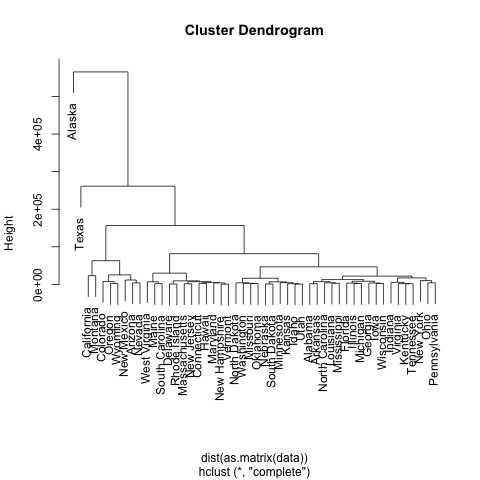
\includegraphics[width=.9\linewidth]{hclust-all-attri-no-scale.png}
\end{center}

\subsection*{Step 3}
\label{sec:orgea78e1c}
\begin{verbatim}
# Repeat the previous item with a normalized dataset and note any differences
png(filename="hclust-all-attri-with-scale.png")
plot(hclust(dist(as.matrix(scale(data)))))
\end{verbatim}

\begin{center}
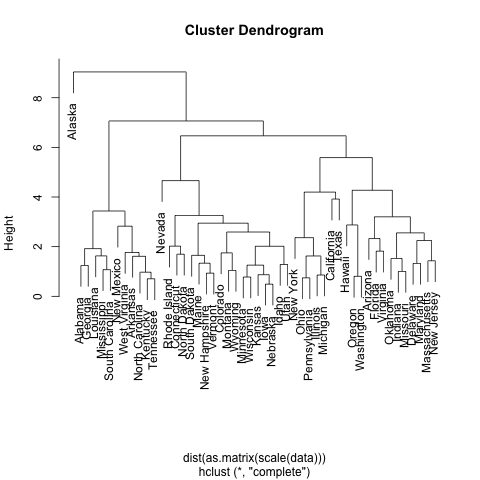
\includegraphics[width=.9\linewidth]{hclust-all-attri-with-scale.png}
\end{center}

The scaled clusters seem to do a much better job of creating distinct clusters.
A heuristic analysis of the dendogram makes it seem that total area of a the
state overpowered nearly all of the other attributes when determining the raw
data. By normalizing it, the other attributes were able to have a stronger
influence on the clusters.
\subsection*{Step 4}
\label{sec:orgbdc12be}
\begin{verbatim}

# Remove "Area" from the attributes and re-cluster (and note any differences)
png(filename="hclust-no-area-with-scale.png")
plot(hclust(dist(as.matrix(
        scale(data[,c("Population", "Income", "Illiteracy",
                 "Life Exp", "Murder", "HS Grad", "Frost")])))))
\end{verbatim}

\begin{center}
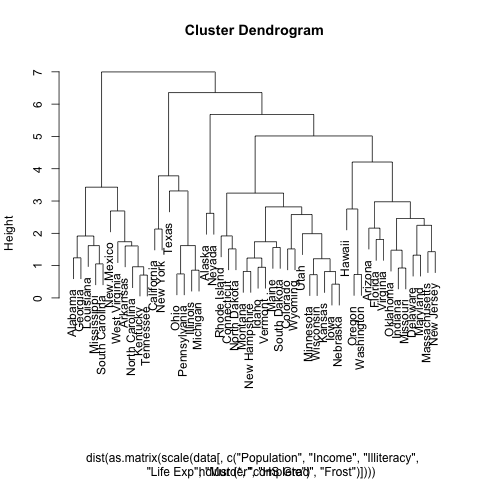
\includegraphics[width=.9\linewidth]{hclust-no-area-with-scale.png}
\end{center}

Without area, the dendogram looks even more balanced. I think this shows just
how disproportionate some of the state sizes are. States with very similar
attributes in every other respect are grouped differently just because one is
much larger than the other. You are now able to see actual regions in the
country being grouped together. 

\subsection*{Step 5}
\label{sec:orgc3bddae}

\begin{verbatim}
# Cluster only on the Frost attribute and observe the results
png(filename="hclust-only-frost-with-scale.png")
plot(hclust(dist(as.matrix(scale(data[,"Frost"])))))
\end{verbatim}

\begin{center}
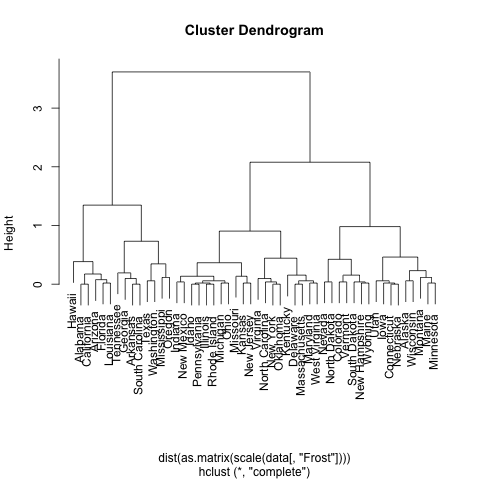
\includegraphics[width=.9\linewidth]{hclust-only-frost-with-scale.png}
\end{center}

I saw pretty close to what I expected. States with similar weather patterns are
grouped together, and often states on similar latitudes are grouped together,
even if they are far apart. 
\section*{USING K-MEANS}
\label{sec:orgdcc63b2}
\subsection*{Step 1}
\label{sec:org130f0b9}
\begin{verbatim}
data <- scale(state.x77)
\end{verbatim}
\subsection*{Step 2}
\label{sec:org2c27125}
\begin{verbatim}
myClusters = kmeans(data, 3)
summary(myClusters)
print(myClusters$centers)
print(myClusters$cluster)
\end{verbatim}
\subsubsection*{Summary}
\label{sec:org178039a}
\begin{verbatim}
# Length Class  Mode
# cluster      50     -none- numeric
# centers      24     -none- numeric
# totss         1     -none- numeric
# withinss      3     -none- numeric
# tot.withinss  1     -none- numeric
# betweenss     1     -none- numeric
# size          3     -none- numeric
# iter          1     -none- numeric
# ifault        1     -none- numeric
\end{verbatim}
\subsubsection*{Mean Values}
\label{sec:orga36e8b5}

\begin{center}
\begin{tabular}{rrrr}
Population & Income & Illiteracy & Life-Exp\\
\hline
-0.2269956 & -1.3014617 & 1.391527063 & -1.1773136\\
-0.4873370 & 0.1329601 & -0.641201154 & 0.7422562\\
0.9462026 & 0.7416690 & 0.005468667 & -0.3242467\\
\end{tabular}
\end{center}

\begin{center}
\begin{tabular}{rrrr}
Murder & HS-Grad & Frost & Area\\
\hline
1.0919809 & -1.4157826 & -0.7206500 & -0.2340290\\
-0.8552439 & 0.5515044 & 0.4528591 & -0.1729366\\
0.5676042 & 0.1558335 & -0.1960979 & 0.4483198\\
\end{tabular}
\end{center}

\subsubsection*{Cluster Assignments}
\label{sec:org8759f22}

\begin{center}
\begin{tabular}{rrrrr}
Alabama & Alaska & Arizona & Arkansas & California\\
3 & 1 & 1 & 3 & 1\\
Colorado & Connecticut & Delaware & Florida & Georgia\\
2 & 2 & 2 & 1 & 3\\
Hawaii & Idaho & Illinois & Indiana & Iowa\\
2 & 2 & 1 & 2 & 2\\
Kansas & Kentucky & Louisiana & Maine & Maryland\\
2 & 3 & 3 & 2 & 1\\
Massachusetts & Michigan & Minnesota & Mississippi & Missouri\\
2 & 1 & 2 & 3 & 1\\
Montana & Nebraska & Nevada & New-Hampshire & New-Jersey\\
2 & 2 & 1 & 2 & 1\\
New-Mexico & New-York & North-Carolina & North-Dakota & Ohio\\
3 & 1 & 3 & 2 & 1\\
Oklahoma & Oregon & Pennsylvania & Rhode-Island & South-Carolina\\
2 & 2 & 1 & 2 & 3\\
South-Dakota & Tennessee & Texas & Utah & Vermont\\
2 & 3 & 1 & 2 & 2\\
Virginia & Washington & West-Virginia & Wisconsin & Wyoming\\
1 & 2 & 3 & 2 & 2\\
 &  &  &  & \\
\end{tabular}
\end{center}
\subsubsection*{Cluster Assignments Plot}
\label{sec:orge1d668d}
\begin{center}
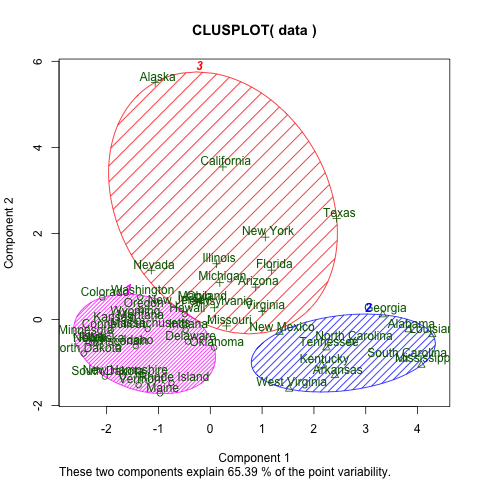
\includegraphics[width=.9\linewidth]{k-3-clusters.png}
\end{center}
\subsubsection*{Analysis}
\label{sec:org7c96fa3}
My guess is that area and population are the largest factors in these grouping.
We can see on the plot that Alaska, California, and Texas are outliers, probably
due to their size/population ratios. 
\subsection*{Step 3}
\label{sec:orgf729d21}
\begin{verbatim}
errors <- c()
for (k in 1:25) {
    errors[k] <- kmeans(data, k)$tot.withinss
}
png("kmeans-sum-squares-error.png")
plot(errors, xlab = "k", ylab = "within-cluster sum of squares error")
\end{verbatim}

\begin{center}
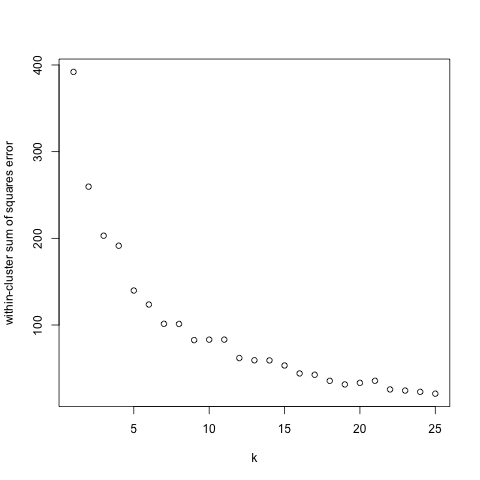
\includegraphics[width=.9\linewidth]{kmeans-sum-squares-error.png}
\end{center}

\subsection*{Step 4}
\label{sec:org451160d}
I picked 10, as it seems like that is when the rate of error stops decreasing
significantly. 
\begin{verbatim}
k <- 10
\end{verbatim}
\subsection*{Step 5}
\label{sec:orgd337082}
\begin{verbatim}
print(cluster$cluster)
\end{verbatim}
\begin{center}
\begin{tabular}{lllll}
 &  &  &  & \\
Alabama & Alaska & Arizona & Arkansas & California\\
4 & 2 & 3 & 4 & 10\\
Colorado & Connecticut & Delaware & Florida & Georgia\\
7 & 1 & 8 & 8 & 4\\
Hawaii & Idaho & Illinois & Indiana & Iowa\\
5 & 7 & 8 & 8 & 7\\
Kansas & Kentucky & Louisiana & Maine & Maryland\\
7 & 4 & 4 & 9 & 8\\
Massachusetts & Michigan & Minnesota & Mississippi & Missouri\\
1 & 8 & 7 & 4 & 8\\
Montana & Nebraska & Nevada & New-Hampshire & New-Jersey\\
6 & 7 & 6 & 9 & 8\\
New-Mexico & New-York & North-Carolina & North-Dakota & Ohio\\
3 & 10 & 4 & 1 & 8\\
Oklahoma & Oregon & Pennsylvania & Rhode-Island & South-Carolina\\
3 & 5 & 8 & 1 & 4\\
South-Dakota & Tennessee & Texas & Utah & Vermont\\
9 & 4 & 10 & 7 & 9\\
Virginia & Washington & West-Virginia & Wisconsin & Wyoming\\
8 & 5 & 4 & 7 & 6\\
\end{tabular}
\end{center}

\subsection*{Step 6}
\label{sec:orgc351224}
\begin{center}
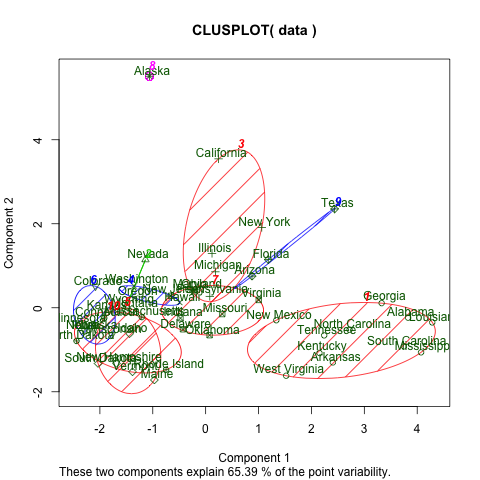
\includegraphics[width=.9\linewidth]{kmeans-10.png}
\end{center}
\subsection*{Step 7}
\label{sec:orgf0e2259}

\begin{center}
\begin{tabular}{rrrr}
Population & Income & Illiteracy & Life-Exp\\
\hline
-0.3499380 & 0.5656501 & -0.7710820 & 1.2544011\\
-0.4514893 & 0.5182516 & 0.0902330 & 0.8353735\\
-0.7660428 & -0.5843829 & -0.9117048 & 0.4809958\\
-0.1667872 & -1.3624751 & 1.8866900 & -1.7868083\\
-0.8429672 & 0.6862826 & -1.0171720 & -0.9077815\\
0.7891560 & 0.5328170 & -0.3117140 & -0.2462765\\
2.8948232 & 0.4869237 & 0.6507713 & 0.1301655\\
-0.2771693 & -1.2506172 & 0.9788913 & -0.6694013\\
-0.8693980 & 3.0582456 & 0.5413980 & -1.1685098\\
-0.3889962 & 0.1472000 & -0.1148420 & 0.3157792\\
\end{tabular}
\end{center}

\begin{center}
\begin{tabular}{rrrr}
Murder & HS-Grad & Frost & Area\\
\hline
-1.1080742 & 0.55150442 & 0.859258777 & -0.058630181\\
-0.4748696 & 0.96161967 & -1.571925102 & -0.001018197\\
-0.9150653 & 0.65342525 & 0.994267293 & -0.099820942\\
1.5933731 & -1.55107136 & -1.213139113 & -0.287006387\\
0.4935610 & 1.35471127 & 1.462846466 & 0.384520782\\
0.3093560 & -0.19041729 & -0.001154271 & -0.342772830\\
1.0172810 & 0.13932569 & -1.131057600 & 0.992720037\\
0.6741541 & -1.30304191 & -0.310242469 & -0.189881160\\
1.0624293 & 1.68280347 & 0.914567609 & 5.809349671\\
\end{tabular}
\end{center}

I see that area, income, and population seem to have the greatest deviation among the
attributes. This suggests they have the greatest influence on the centers due
to the nature of Euclidean distance. The rest of the attributes do not have
nearly as much of a range, indicating they do not have a large influence on
the centers in comparison.

\section*{Summary}
\label{sec:orga7ca44c}
D). I completed all of the steps.
\end{document}
